\scanpage{327}
$X$ courbe alg. $/\mathbb C$ \unsure{propre non sing connexe}, genre $g\geq2$.
Il y a sur $X$ un \deleted{fibré principal}\inserted{torseur} canonique
$P$ de \unsure{gr.} $\mathrm{GP}(1)_{\mathbb C}=G'_{\mathbb C}$ à connexion intégrable
(compatible à structure de torseur), obtenu ainsi:
$\forall x\in X\longmapsto\widetilde X(x)$ rev. universel de $X$ en $x$
\[
\widetilde X(x)\unsure{\longleftrightarrow|\simeq}
\deleted{\unsure{demi-plan disque}}\inserted{demi-plan de}\text{ Poincaré }D
\]
ens. des iso $\operatorname{Iso}\bigl((D,0),\widetilde X(x,\widetilde x)\bigr)$ est un torseur à droite
sur $\unsure{\widehat{\operatorname{Isot}}|\operatorname{Isot}}(D,0)\simeq
\deleted{\mathrm{GP}(1)_{\mathbb R}\simeq G'_{\mathbb C}}\inserted{S_{\mathbb R}}$,
d'où par \unsure{ext.} un torseur à droite sur $G'$, \inserted{soit $P_x$.}
\deleted{\unsure{ceci dit par $G_0$}}.
\margin{\unsure{On}}

On \unsure{sait|voit} que les $P_x$ ($x\in X(\mathbb C)$) sont les fibres
d'un fibré principal \deleted{analytique}\inserted{top.} à structure \unsure{plat|plate}
(celui associé à $\pi_{\unsure{x|1}}\longrightarrow G'_{\mathbb R}\subset G'_{\mathbb C}$)

\uline{Th} $\forall x\in X$, $\exists$ une et une seule \deleted{\unsure{imm.}}\inserted{\unsure{imm.}}
\unsure{ouverte} analytique de $\widetilde X(x)$ dans
$T_x(X)$ dont a) l'image est un disque
b) l'application tangente en $\widetilde x$ est l'identité.
\figure{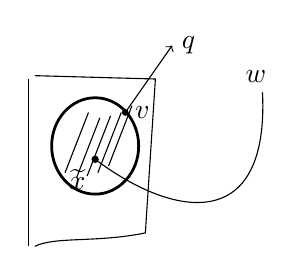
\begin{tikzpicture}[scale=.85]
\draw (0,0)--(0,2.5);\draw (.1,2.55)--(1.9,2.5)--(1.75,.2).. controls (1,.05) and (.4,.15) .. (.1,0);
\draw[line width=1pt] (1,1.5) ellipse (.65 and .72);
\foreach \x/\y in {.55/1.1,.72/1.02,.88/1.05,1.04/1.1,1.2/1.2}{\draw (\x,\y)--(\x+.35,\y+.9);}
\fill (1,1.3) circle (.055);\node[below left] at (1,1.3) {$\widetilde x$};
\fill (1.45,2) circle (.05);\node[right] at (1.45,2) {$\unsure{v}$};
\draw[->] (1.45,2)--(2.15,3);\node[right] at (2.15,3) {$\unsure{q}$};
\draw (1,1.3) .. controls (2.2,.4) and (3.6,.2) .. (3.5,2.3);\node[above] at (3.4,2.3) {$\unsure{w}$};
\end{tikzpicture}}
\[
\pi_1(X,x)\subset G'\subset G'_{\mathbb C}
\]
\figure{\begin{tikzpicture}\draw[->] (0,.6)--(.1,0);\node[below] at (.1,0) {$\unsure{u}$};\end{tikzpicture}}
\[
\begin{pmatrix}a&b\\c&d\end{pmatrix}\mathbin{.}z=
\qquad
\begin{array}{cc}a^{\unsure{*}}&b\\-b&a\end{array}
\]
\[
\deleted{\unsure{\mathrm{Iso}}}\uline{P(x,q)}
\]
\[
P(x,\varphi q)=P(x,q)\mathop{\wedge}_{i_{\varphi}}G'_{\mathbb C}
\]
\[
\unsure{\varphi\in S'_{\mathbb C}\subset G'\subset G'_{\mathbb C}}
\qquad\mathbb C^*
\]
\diagram{\begin{tikzcd}
P(x,q)\arrow[d,"\unsure{z}"']&G'_{\mathbb C}\arrow[d,"\unsure{i_{\varphi}}"]\\
P(x,\unsure{x'|u'})&G'_{\mathbb C}
\end{tikzcd}}
\diagram{\begin{array}{ccc}
Q_{\mathbb R}& &\textcircled{$P_{\mathbb R}$}\\
&S_{\mathbb R}\subset&G'_{\mathbb R}\\
&\cap&\cap\\
Q_{\mathbb C}&S_{\mathbb C}\subset&G'_{\mathbb C}\quad P_{\mathbb C}
\end{array}}
\figure{\begin{tikzpicture}
\draw (.4,2.5).. controls (-.2,2) and (-.2,1.4) .. (.3,1);
\draw (0,.3)--(0,0)--(3,0)--(3.05,.3);
\end{tikzpicture}}
\margin{$P(x,\varphi\unsure{q})=P(x,\unsure{x|u})\mathop{\wedge}_{i_{\varphi}}G'_{\mathbb C}$}
\diagram{\begin{tikzcd}
\mathbb C^*\subset\mathrm{G\ell}(2,\mathbb R)\arrow[d]\\
\mathrm{G\ell}(2,\mathbb C)
\end{tikzcd}}
\margin{$G_m\longrightarrow\unsure{\mathrm{GP}_{\mathbb R}|\mathrm{GP}_2}$}
\diagram{\begin{tikzcd}E\arrow[r]&E\otimes\Omega\end{tikzcd}}
\figure{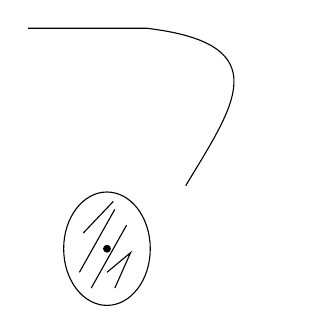
\begin{tikzpicture}
\draw (0,2)--(1.5,2) .. controls (3.2,1.8) and (2.6,1) .. (2,0);
\draw (1,-.8) ellipse (.55 and .72);
\fill (1,-.8) circle (.05);
\draw (.65,-1.1)--(1.1,-.3);\draw (.8,-1.3)--(1.25,-.5);\draw (.7,-.6)--(1.08,-.2);\draw (1,-1.1)--(1.3,-.85)--(1.1,-1.3);
\end{tikzpicture}}
\diagram{\begin{tikzcd}E\arrow[r]&E\otimes\Omega\end{tikzcd}}

 a) fibré inversible: $\uline{\Omega^{-1}}$

 b) \deleted{\unsure{fibré}} $\mathrm P(\Omega^{-1}+\Omega)$ avec conn. intégrable
\[
\begin{pmatrix}\Omega&0\\\Omega^3&\Omega\end{pmatrix}
\]
\figure{\begin{tikzpicture}\draw (0,2)--(2,2).. controls (2.7,2) and (2.4,.8) .. (3,0);\end{tikzpicture}}
\[
\boxed{\begin{gathered}
\text{Trouver une connexion intégrable}\\
\text{(alg) canonique sur}\\
\mathrm P(\Omega^{-1}+\Omega)=\overline{\mathrm V(\Omega^2)}
\end{gathered}}
\]
\[
\Omega^{-1}\oplus\Omega\longrightarrow(\Omega^{-1}\oplus\Omega)\otimes\Omega
=\unsure{\Omega_X^0|\mathcal O_X}+\Omega^2
\]
\[
\unsure{(D,\omega)=(d,\overline\omega,\Delta)}
\]
\figure{
\begin{tikzpicture}\draw[line width=1pt] (0,0)--(.1,.65);\end{tikzpicture}}
\margin{328}
